\documentclass{article}



% \usepackage{arxiv}
\RequirePackage[colorlinks,citecolor=blue,urlcolor=blue,allcolors=blue]{hyperref}
\usepackage[utf8]{inputenc} % allow utf-8 input
\usepackage[T1]{fontenc}    % use 8-bit T1 fonts
\usepackage{url}            % simple URL typesetting
\usepackage{booktabs}       % professional-quality tables
\usepackage{amsfonts}       % blackboard math symbols
\usepackage{nicefrac}       % compact symbols for 1/2, etc.
\usepackage{microtype}      % microtypography
\usepackage{lipsum}		% Can be removed after putting your text content
\usepackage{graphicx}
\usepackage{natbib}
\usepackage{doi}
\usepackage{amsmath,amsthm,amssymb,scrextend,mathtools}
\usepackage{xr}
\externaldocument{bayesian_stack_arxiv}
% \RequirePackage[colorlinks,citecolor=blue,urlcolor=blue]{hyperref}


\newtheorem{theorem}{Theorem}
\newtheorem{lemma}{Lemma}
\newtheorem{definition}{Definition}
\usepackage{natbib}
\usepackage{lmodern} %%helps deal with font size problems
\usepackage{dsfont}
\newcommand{\1}[1]{\mathds{1}\left[#1\right]}

\newcommand{\spencer}[1]{{\color{red} Spencer: #1}}
\newcommand{\jarad}[1]{{\color{white} Jarad: #1}}



% \title{Supplemental Material for Bayesian stacking via proper scoring rule
% optimization using a Gibbs
% posterior}
% \shorttitle{Quantile Gaussian Process Matching}

%\date{September 9, 1985}	% Here you can change the date presented in the paper title
%\date{} 					% Or removing it



% Uncomment to remove the date
% \date{}

% Uncomment to override  the `A preprint' in the header
% \renewcommand{\headeright}{}
%\renewcommand{\undertitle}{Technical Report}
% \renewcommand{\shorttitle}{Stacked Gibbs Posterior, Supplement}

%%% Add PDF metadata to help others organize their library
%%% Once the PDF is generated, you can check the metadata with
%%% $ pdfinfo template.pdf
% \hypersetup{
% pdftitle={A template for the arxiv style},
% pdfsubject={q-bio.NC, q-bio.QM},
% pdfauthor={David S.~Hippocampus, Elias D.~Striatum},
% pdfkeywords={First keyword, Second keyword, More},
% }

\begin{document}
% \maketitle
% 

% 
% 
% % keywords can be removed
\Huge
\begin{center}
Supplemental Material for Bayesian stacking via proper scoring rule
optimization using a Gibbs
posterior
\end{center}

\normalsize
\section{Additional plots from first simulation study}

When optimizing linear pool model weights for adaptive variable AVS
in the i.i.d. data simulation study in section 4.1, the learning rate $\eta$
was selected via LOO cross validation. In the study, data
was simulated from the specified mixture model for sample sizes
$n \in \{10, 20,50, 100, 200\}$. 
For each sample size, there were 500s replicates. 
In each replicate, the AVS linear pool was fit using each of 30 equally spaced
values of the potential learning rate $\eta$ from 0.001 to 1.5.
Each of the $n$ observations was left out in turn, and the 
AVS linear pool was fit using the remaining $n-1$ data points. The CRPS
was then computed for the held out point. The value $\eta_i^*$ was set 
as learning rate value which minimized the CRPS.
Finally, the learning rate $\eta$ was set as the mean of the $n$ $\eta_i^*$s,
and the AVS was fit using all $n$ data points with $\eta$ as the learning rate.
The left plot in figure \ref{fig:min_etas} shows an example of the CRPS
values over each of 30 grid points when the sample size is $n = 10$.

\begin{figure}[hbt!]
\centering
%\begin{subfigure}{}
  % \centering
  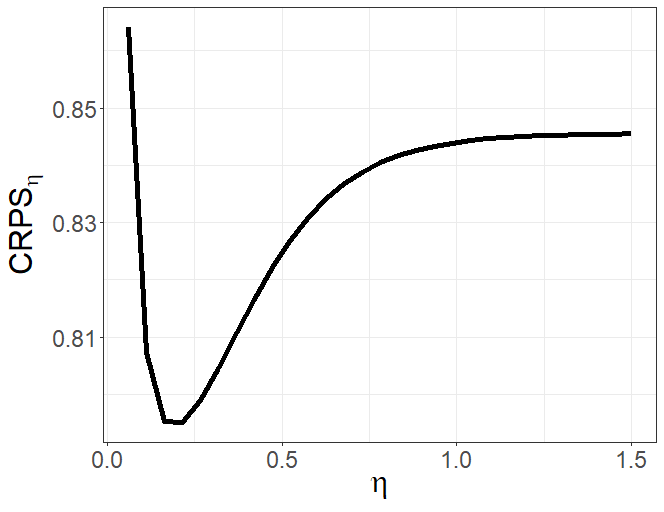
\includegraphics[width=.48\linewidth]{Images/avs_eta_min.png}
  % \caption{A subfigure}
  % \label{fig:sub1}
%\end{subfigure}%
%\begin{subfigure}{}
  \centering
  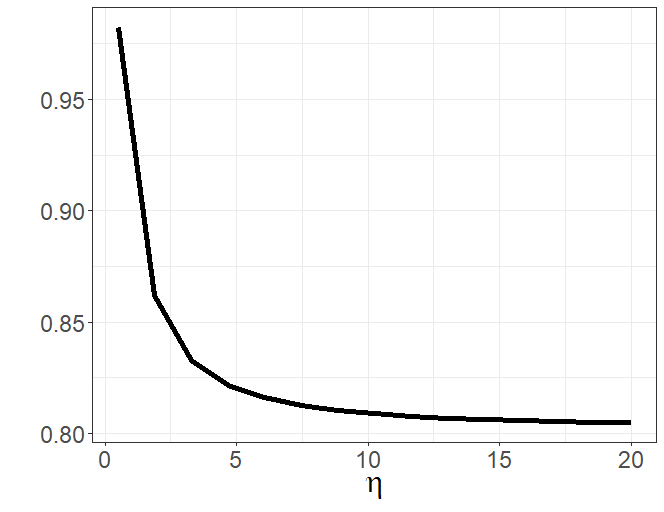
\includegraphics[width=.48\linewidth]{Images/sgp_eta_min.png}
  % \caption{A subfigure}
  % \label{fig:sub2}
%\end{subfigure}
\caption{An example of CRPS values for different values of $\eta$ after 
optimizing competing model weights for AVS (left) and for SGP (right).}
\label{fig:min_etas}
\end{figure}

\newpage
\section{Additional plots from second simulation study}

\begin{figure}[hbt!]
\centering
%\begin{subfigure}{}
  % \centering
  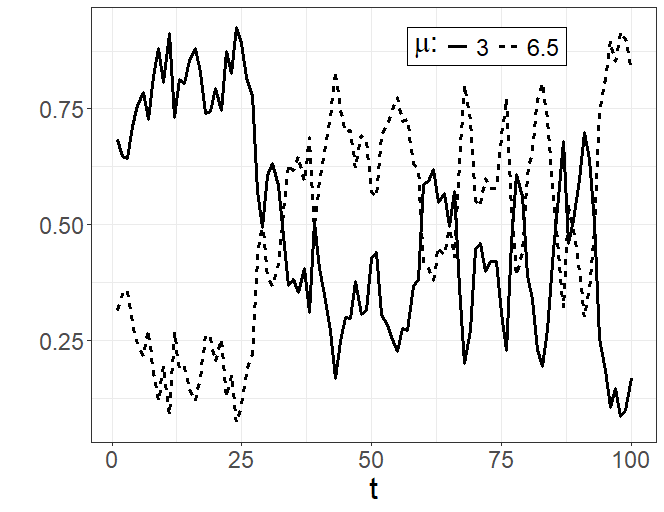
\includegraphics[width=.48\linewidth]{Images/dyn_wts_tr_ex.png}
  % \caption{A subfigure}
  % \label{fig:sub1}
%\end{subfigure}%
\hspace{0.01\textwidth}
%\begin{subfigure}{}
  \centering
  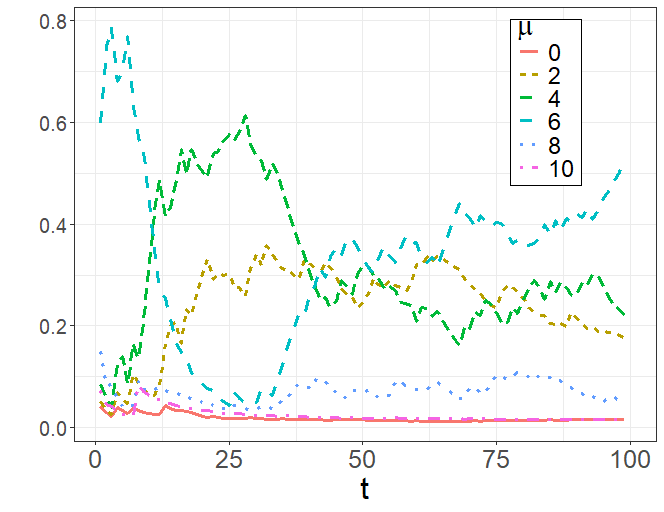
\includegraphics[width=.48\linewidth]{Images/dyn_wts_opt_ex.png}
  % \caption{A subfigure}
  % \label{fig:sub2}
%\end{subfigure}
\caption{An example of simulated component weights for 100 time steps. 
The figure shows the simulated weights for the two components of the true 
distribution (left) and the weights optimized under SGP for the six competing 
component models (right).}
\label{fig:dyn_wts_ex}
\end{figure}


\newpage
\section{Additional plots from third simulation study}
\begin{figure}[hbt!]
\centering
  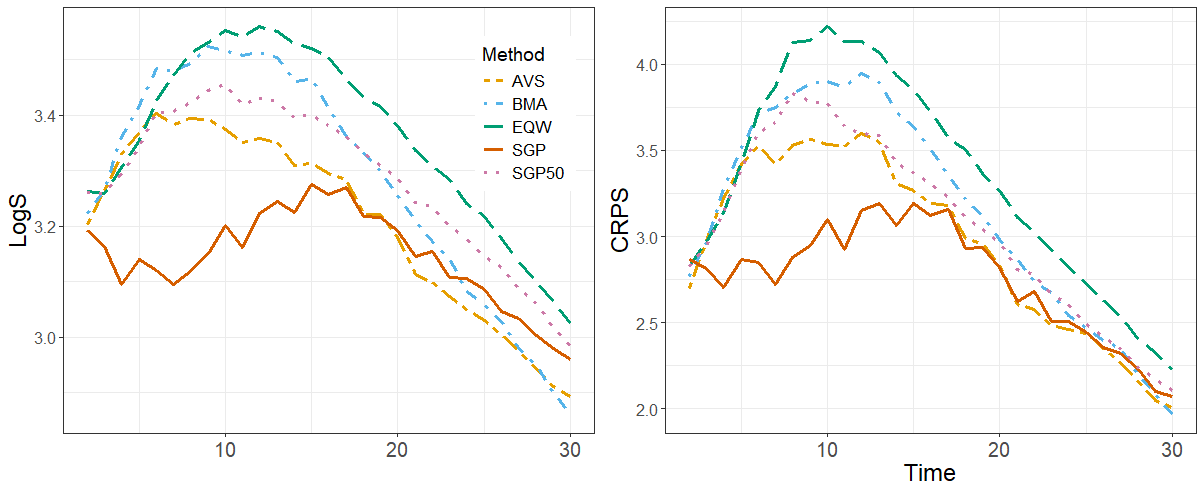
\includegraphics[width=.98\linewidth]{Images/sir_sim_med_col.png}
\caption{Plots showing results for one step ahead forecasts for SIR
data for the four
weighting methods SGP, AVS, BMA, and EQW. The median LogS (left) and 
CRPS (right) over 3,000 replicates of one step
ahead predictions at 29 time points colored by weighting methods.
}
\label{fig:sir_sim_med}
\end{figure}



\begin{figure}[hbt!]
\centering
  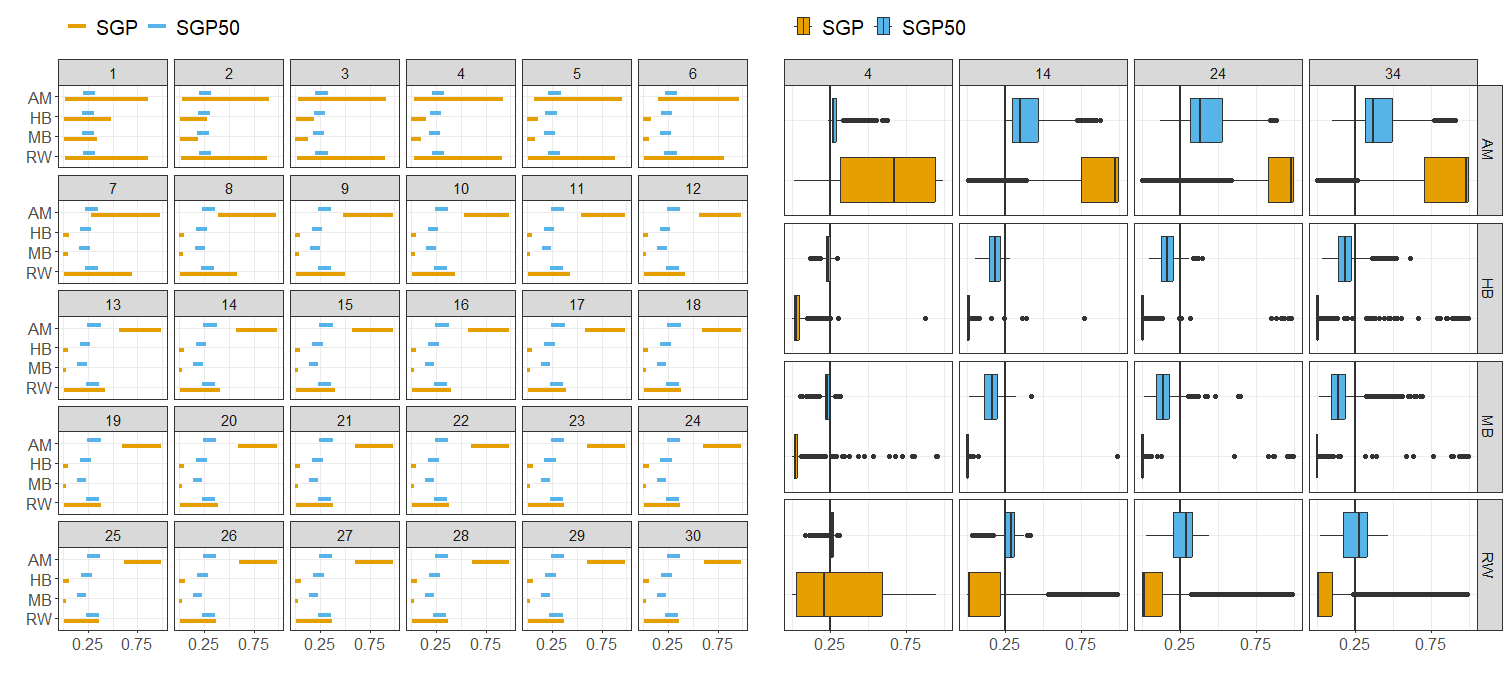
\includegraphics[width=.98\linewidth]{Images/sir_post_res.png}
\caption{Plots showing results of posterior weights for SGP and SGP50.
 95\% credible intervals for SGP and SGP50 
weights for 30 time steps
of 1 simulation replicate from simulation study (left) and 
boxplots of mean posterior weights for each component model for selected
time steps 4, 14, 24, and 34 for all 3,000 replicates faceted by 
time step and component model (right). The four component forecast models are
the ARIMA (AM), hierarchical Bayesian (HB), Bayesian mechanistic SIR (MB), and
random walk (RW).
}
\label{fig:sir_post_res}
\end{figure}


\newpage

\section{Weighted interval score results from 2023 FluSight forecast analysis}

\begin{figure}[hbt!]
\centering

  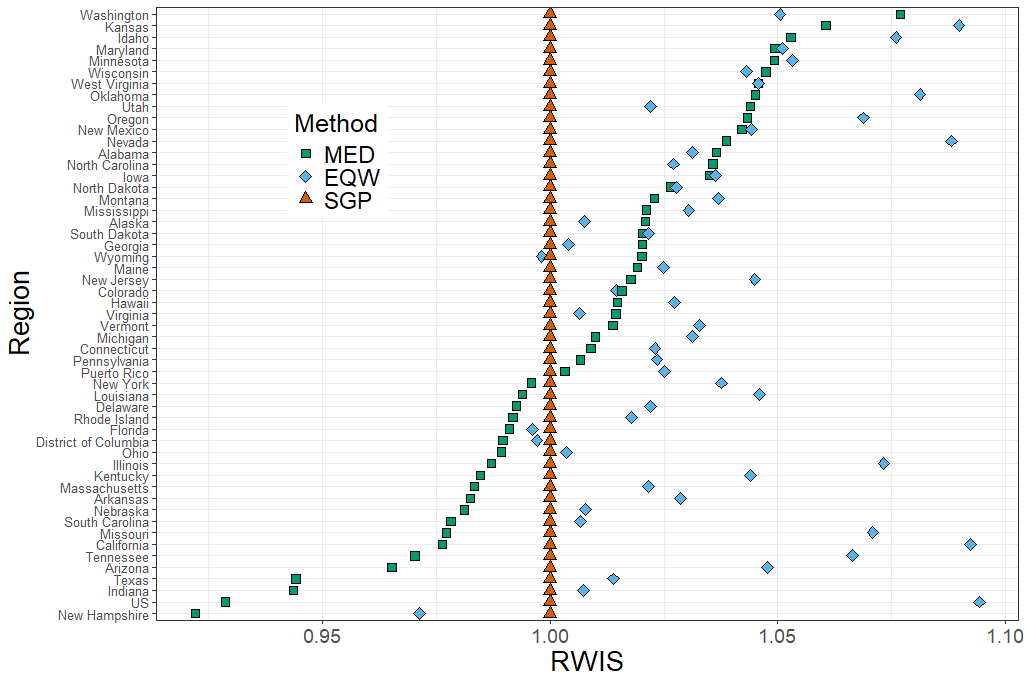
\includegraphics[width=.6\linewidth]{Images/flu_region_wis_col.png}
\caption{
Mean over regions WIS for the four ensemble methods divided
by mean WIS for the SGP
separated by shape and color.}
\label{fig:flu_wis}
\end{figure}


\begin{table}[h!]
\centering
\caption{Table showing the number of times ensemble forecasts for each method, 
SGP, AVS, BMA, and EQW, were ranked 1st, 2nd, 3rd, and 4th according to mean 
CRPS by region or week. There were 53
regions evaluated and 29 weeks, so each column under region should sum to 53
and each column under week to 29.}
 \begin{tabular}{cccccccc}
 % {@{\extracolsep{\fill}}
 %    l
 %    *{8}{c}
 %    S[table-format=4.0]}
 \\
  Ranking
  & \multicolumn{3}{c}{By region CRPS}
  &
  & \multicolumn{3}{c}{By week CRPS} \\
  \cmidrule{2-4}  \cmidrule{6-8}
  & MED & EQW & SGP & & MED & EQW & SGP\\
  \midrule
  $1^{st}$ & 21 & 1  & \textbf{31} & & 11 & 1  & \textbf{17}\\
  $2^{nd}$ & 22 & 12 & 19          & & 15 & 9  & 5\\
  $3^{rd}$ & 10 & 40 & 3           & & 3  & 19 & 7\\
  \bottomrule
 \end{tabular}
 \label{tab:forecast_rank_wis}
\end{table}



% \bibliographystyle{unsrtnat}
% \bibliography{master_bib}  %%% Uncomment this line and comment out the ``thebibliography'' section below to use the external .bib file (using bibtex) .



\end{document}
